When it comes to probabilistic forecasting, there are a couple of standard practical approaches; conceptually they can be grouped into two main categories. The former class of approaches tries modelling the distribution of the observed data directly. The latter family of approaches constructs first a point forecast and then learns the distribution of the model's errors.
\section{Quantile regression}
Quantile regression can be interpreted as an extension of standard regression. In this setting, you basically slice the dependent variables into quantiles and then fit a regression for each quantile. With standard regression, we build a model for the conditional mean, conversely, with quantile regression we model the conditional quantile function for any desired quantile. 
Therefore, with quantile regression we are able to study the impact of covariates on quantiles directly.
\begin{definition}
    For any real valued random variable Y, we define its associated quantile function.
    \begin{equation}
        Q_q=\inf\{y:F(y)\geq q\}
    \end{equation}
\end{definition}
Alternatively, in order  to ease the posing of the quantile regression problem, we can formulate quantiles as the solutions to the following optimization problems.
\\
For any $0<q<1$ consider the pinball loss function from section \ref{pinball}, $\rho_q(u)=u(q-\mathbb{I}_{\{u<0\}})$. 
Such loss is minimized by the quantile $Q(q)$.
Thus,we can estimate quantiles by minimizing the expectation of $\rho_q(y-g(x,\beta))$ with respect to the parameter $\beta$.
\\
Note, that in the special case $q=\frac{1}{2}$,  quantile regression corresponds exactly to standard regression with an absolute value loss function.
\\
It follows that the conditional linear quantile function $\hat{Q}_q=x_i\beta(q)$, can be estimated by solving
\begin{equation}\label{eq:linear_quantile_regression_minimisation_problem}
    \hat{\beta}(q)=\argmin{\beta}\sum\limits_{i=1}^n \rho_q   (y_i-x_i \beta)
\end{equation}
\\
Notice that, this cost function is not differentiable, therefore there is no analytical solution to the quantile regression problem. Nevertheless, we can easily solve it by employing linear programming and convex optimisation \cite{boyd2004convex}.
\\
Furthermore, we can extend this framework to non linear quantile regression by choosing a non linear model in place of $x\beta$ in the above equation \ref{eq:linear_quantile_regression_minimisation_problem}.
% \\
% In order to illustrate the approach, let us consider applying quantile regression to the maximum daily temperature dataset in Melbourne \cite{hyndman1996estimating}; models considered will be linear, gradient boosting machine, quantile forest\cite{meinshausen2006quantile} and kernel quantile regression.
% - se si puo fare plot con stessi dati ma differenti f nel quantile regression

% \section{Copula models}
\section{Quantile forest}
Meinshausen \cite{meinshausen2006quantile} extends the idea of random forest \cite{breiman2001random} generalising it, the result is the quantile forest algorithm. Quantile forest allows us to estimate conditional quantiles in a non parametric fashion.
\\
In order to understand this algorithm, it is first necessary to first cover the theory of decision trees and random forests.
\subsection{Decision trees}
Decision trees methods partition recursively the feature space in a set of binary rectangles and then fit a simple model in each of those partitions (the most straightforward is fitting just a constant).
To get started, we first split the space into two disjoint regions, then we model the response variable by the mean of the observed predicted variables with associated features falling in that specific region. Our goal is selecting the best features and best split point such that to achieve the best generalizing fit.
For an example/visualisation consider the pictures \ref{fig:elements_statistical_learning1} and \ref{fig:elements_statistical_learning2} taken from \cite{hastie2009elements}, where the decision tree algorithm is visualised for a regression problem with two independent variables $X_2$ and $X_1$.
\begin{figure}
    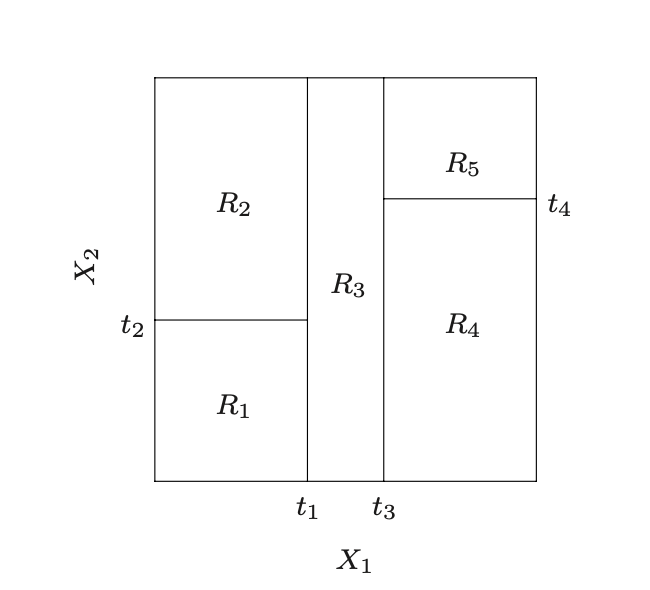
\includegraphics[width=0.5\textwidth]{images/elsii1.png}
    \caption{two-dimensional feature space partitioned by recursive binary splitting}
    \label{fig:elements_statistical_learning1}
  \end{figure}
\\
\begin{figure}
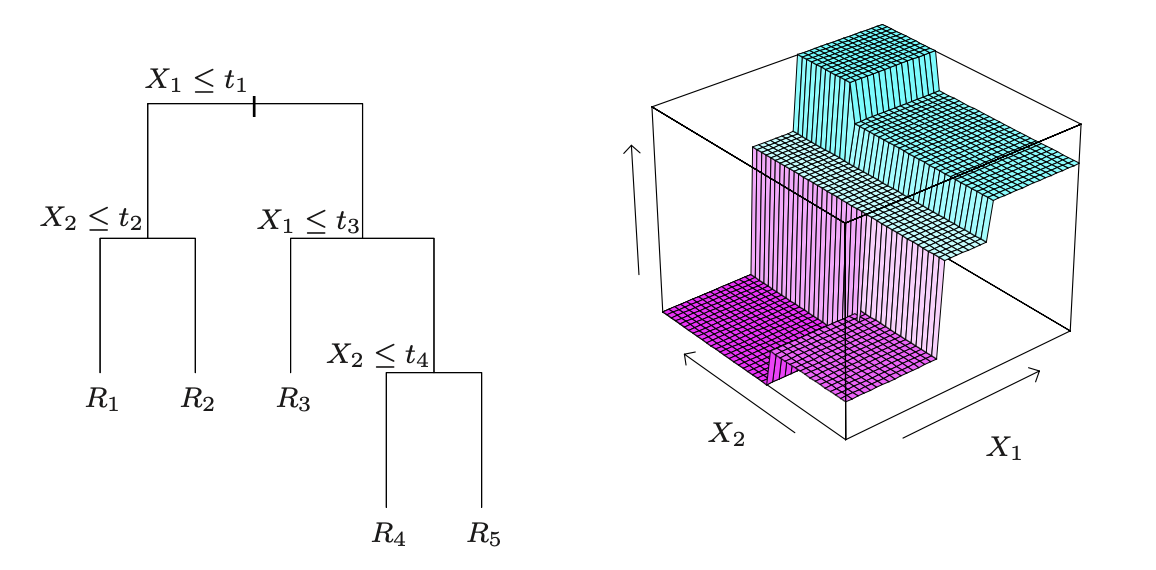
\includegraphics[width=1\textwidth]{images/elsii2.png}
\caption{partition tree and regression model}
\label{fig:elements_statistical_learning2}
\end{figure}
\\
Suppose to partition the feature space into M regions $R_1,\dots,R_M$, then the model reads as follows.
\begin{equation}
    f(x)=\sum\limits_{m=1}^{M}c_m\mathbb{I}_{\{x \in R_m\}}
\end{equation}
\\
It follows that the function minimising the sum of squares is the one with $\hat{c}_m=mean(y_i|x_i \in R_m)$.
Finding the best split in terms of minimum sum of squares is computationally infeasible in practice. Therefore we approximate a solution by approaching the problem in a greedy fashion.
Let $j$ denote the splitting variable and $s$ be the the split point we define the two half planes
\begin{equation}
    R_1(j,s)=\{X|X_j\leq s\} \quad R_2(j,s)=\{X|X_j\>s\}
\end{equation}
Then we search for the $s$ and $j$ that solve
\begin{equation}
    \min_{j,s}\left[\min_{c_1} \sum\limits_{x_i \in R_1(j,s)}(y_i-c_1)^2+\min_{c_2} \sum\limits_{x_i \in R_2(j,s)}(y_i-c_2)^2\right]
\end{equation}
The inner problem is easy, as already pointed out we will have 
\begin{equation}
    \hat{c}_1=mean(y_i|x_i \in R_1) \quad \hat{c}_2=mean(y_i|x_i \in R_2)
\end{equation}
For the outer problem, we scan through all the (j,s) tuples and pick the best pair. 
Next, one or both of these regions from the previous step are split into two more regions; we recurse this process until some stopping condition is triggered (max number of branches, max deth of tree, threshold on the MSE, minimum number of observation in each leaf node).
Notice, this being a greedy algorithm implies that our final solution is guaranteed to be just a local optimum not a global one.
Even though their simplicity, these models have proved themselves to be really powerful. See figure \ref{fig:decision_tree} for a example where decision tree with different hyperparameters are fitted to a sine wave plus noise. The most popular among these model is the CART \cite{breiman2017classification} tree, its name comes from the fact that it can handle both classification and regression problems.
\begin{figure}
    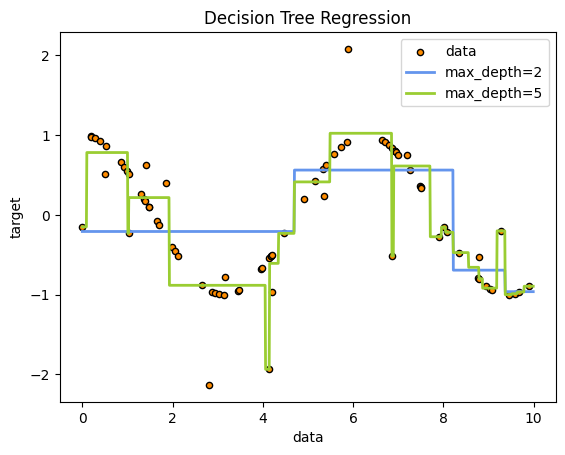
\includegraphics[width=\textwidth]{images/decision_tree.png}
    \caption{decision tree regression}
    \label{fig:decision_tree}
    % image generated on coolab to be quick
\end{figure}
    
\subsection{Bootstrap}
The idea behind boostrapping is to randomly sample from the training set with replacement B times and then fitting B models to each of the "artificial" datasets. Boostrapping can serve different tasks; we can use it to assess the accuracy of a parameter estimate or of a prediction but also to improve their estimates.

\subsection{Bagging}
Bagging stands for boostrap aggregation. 
The bagging estimate is dafined by $\mathbb{E}_P[\hat{f}^*]$ where $P$ is the empirical distribution putting equal probability on each data point of the training set.
Basically, for each bootstrap fitted model $\hat{f}^{*b}(x)$, we compute the bagging estimate by
\begin{equation}
    \hat{f}_{bag}(x)=\frac{1}{B}\sum\limits_{b=1}^{B}\hat{f}^{*b}(x)
\end{equation}
Bagging is particularly useful in reducing the variance of decision trees, resulting in an improved prediction(tradeoff bias variance).
Note, this improvement comes from the fact that averaging reduces variance and leaves biases unchanged.

\subsection{Random forest}
Decision trees are characterised by high variance and low bias, thus, they can benefit extremely from bagging. Furthermore, every decision tree generated through bagging will be identically distributed (i.d.), thus the expectation of an average of B trees is probabilistically equivalent to the expectation of any such trees. As a consequence, the bias will stay fixed since the bias of the bagged estimator is the same as that of each individual tree. 
\\
Consider positively correlated i.d. random variables, then the variance of their average is 
\begin{equation}
    \rho \sigma^2+\frac{1-\rho}{B}\sigma^2
\end{equation}
The second term disappears as B increases, while the first term depends heavily on the correlation between bagged trees. Random forest consists in is reducing the correlation between the trees by randomly selecting m of the p features as candidates for splitting; m tipically takes a value in the order of $\sqrt{p}$ or even 1 with default value $m=\left\lfloor \frac{p}{3} \right\rfloor$, while a good minimum node size is around five. 
\\
Letting $T(x;\Theta_b)$ be the bth bagged tree where $\Theta_b$ denotes the randomness characterizing its splits, cutpoints and terminal node values, we have that the random forest regressor is given by
\begin{equation}
    \hat{f}_{rf}^{B}=\frac{1}{B}\sum\limits_{b=1}^{B}T(x;\Theta_b)
\end{equation}
For a simple visualisation compare figure \ref{fig:random_forest} with \ref{fig:decision_tree}
\begin{figure}
    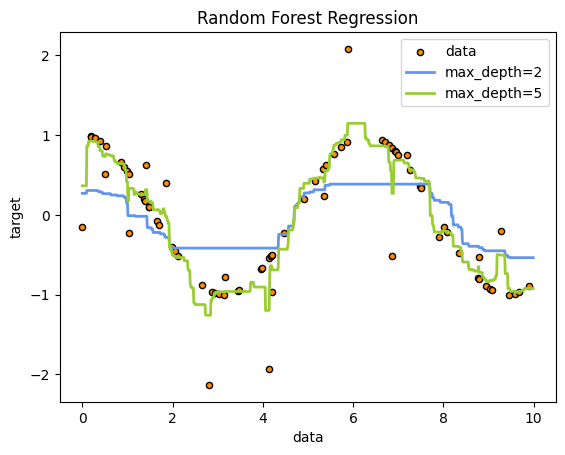
\includegraphics[width=\textwidth]{images/random_forest.png}
    \caption{random forest regression}
    \label{fig:random_forest}
    % image generated on coolab to be quick
\end{figure}


\subsection{Quantile forest}
The key observation here is noting that random forests approximates the conditional mean $\mathbb{E}(Y|X=x)$ by a weighted average over the observed $Y$. Hence, we can extend this idea to the full conditional distribution by
\begin{equation}
    F(y|X=x)=P(Y\leq y|X=x)=\mathbb{E}(\mathbb{I}_{\{Y\leq y\}}|X=x)
\end{equation}
All we have to do is approximating $\mathbb{E}(\mathbb{I}_{\{Y\leq y\}}|X=x)$ by a weighted mean over the random variable $\mathbb{I}_{\{Y\leq y\}}$
\begin{equation}
    \hat{F}(y|X=x)=\sum\limits_{i=1}^{n}\omega_i(x)\mathbb{I}_{\{Y_i\leq y\}}
\end{equation}
By swapping $F(y|X=x)$ with $\hat{F}(y|X=x)$ in the defintion of conditional quantiles we obtain their respective random forest estimator
\begin{equation}
    \hat{Q}_q=\inf\{y:\hat{F}(y|X=x)\geq q\}
\end{equation}


\section{Quantile gradient boosting machine}
\subsection{Boosting}
With boosting we fit an additive expansion of elementary basis functions; with M basis functions we have 
\begin{equation}
    f(x)=\sum\limits_{m=1}^{M}\beta_m b(x;\gamma_m)
\end{equation}
where $b(x;\gamma)$ are the basis functions while $\beta_m$ are the coefficients of the expansion.
Boosted models are fitted by minimizing a loss function over the training data
\begin{equation}
    \min_{\beta_m, \gamma_m}\sum\limits_{i=1}^{N}L\left(y_i, \sum\limits_{m=1}^M \beta_m b(x_i;\gamma_m)\right)
\end{equation}
However, such problem is highly intensive in terms of computation. Therefore, what is done in the literature is approximating its solution by iteratively adding new basis function to the current expansion. That is, we construct $f_m$ by solving for the optimal basis function and coefficients to add to $f_{m-1}$. Considering the square loss, we would have
\begin{equation}
    L(y_i, f_{m-1}(x_i)+\beta_m b(x_i;\gamma))=(e_{im}-\beta_m b(x_i;\gamma))^2
\end{equation}

\subsection{Boosted trees}
We combine several trees obtaining the boosted tree model
\begin{equation}
    f_M(x)=\sum\limits_{m=1}^M T(x;\Theta_m)
\end{equation}
Thus, at each step of the iterative optimisation procedure, we have to solve
\begin{equation}\label{boosting_minimisation_problem}
    \hat{\Theta}_m=\argmin{\Theta_m}\sum\limits_{i=1}^{N}L(y_i, f_{m-1}(x_i)+T(x_i;\Theta_m))
\end{equation}
Remember, $\Theta_m$ referes to the parameters of the mth tree, $\Theta_m=\{R_{jm}, \gamma_{jm}\}_1^{J_m}$
\subsection{Gradient boosting}
In order to robustly solve \ref{boosting_minimisation_problem}, gradient boosting considers the following problem
\begin{equation}
    \tilde{\Theta}_m=\argmin{\Theta}\sum\limits_{i=1}^{N}\left(-g_{im}-T(x_i;\Theta)\right)^2
\end{equation}
where $g_{im}$ is the gradient of $L(f)=\sum\limits_{i=1}^N L(y_i, f(x_i))$ evaluated at $f_{m-1}$. Put simply, we are fitting the m-th tree to the negative of the gradient values of f through least squares.
In order to solve our quantile regression tasks through gradient boosting, all we need to do is specifying the pinball loss as our criterion to guide the minimisation algorithm. See figure \ref{fig:gradient_boosting} for a visualisation
\begin{figure}
    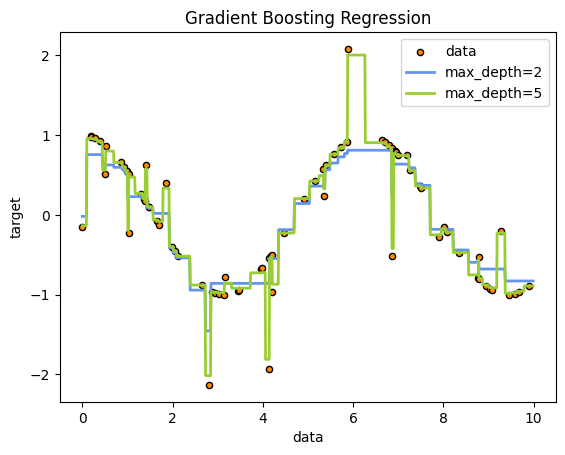
\includegraphics[width=\textwidth]{images/gradient_boosting.png}
    \caption{gradient boosting regression}
    \label{fig:gradient_boosting}
    % image generated on coolab to be quick
\end{figure}



\section{Kernel methods}
\subsection{Kernel quantile regression}
The idea of quantile regression has been extended to kernel methods by Takeuchi et al. \cite{takeuchi2006nonparametric}.
There, they minimize a risk plus regularizer defined as follows.
\begin{equation}\label{eq:kqr_min1}
    R[f]:=\frac{1}{m}\sum\limits_{i=1}^{m}\rho_q(y_i-f(x_i))+\frac{\lambda}{2}\|g\|_\mathcal{H}^2
\end{equation}
where $f=g+b$, $g \in \mathcal{H}$ and $b \in R$.
Using the link between RKHS and feature spaces, we can rewrite $f(x)=\langle w, \phi(x) \rangle+b$. Moreover, note that the RKHS norm is defined as follows $\|f\|_{\mathcal{H}}=\inf\{\|w\|_{F}:w\in F,f(x)=\langle w,\varphi (x)\rangle _{F},\forall x\in X\}$, where $F$ is the feature space.
 Doing so we obtain a minimization problem equivalent to minimizing equation \ref{eq:kqr_min1}.
\begin{equation}\label{eq:kqr_min2}
    \begin{aligned}
    \min_{w,b} \quad & C \sum \limits_{i=1}^{m}
    q(y_i-\langle w, \phi(x) \rangle-b)+ (1-q)(-y_i+\langle w, \phi(x) \rangle+b)+ \frac{1}{2}\|w\|^2\\
    \end{aligned}
    \end{equation}
Note the division by $\lambda$ so that $C=\frac{1}{\lambda m}$.
\\
We can next rephrase the optimisation in \ref{eq:kqr_min2} by introducing the slack variables $\xi_i$ and $\xi_i^*$.
\begin{equation}\label{eq:kqr_min3}
    \begin{aligned}
        \min_{w,b,\xi_i,\xi_i^*} \quad & C \sum \limits_{i=1}^{m}
        q \xi_i+ (1-q)\xi_i^*+ \frac{1}{2}\|w\|^2\\
    \textrm{s.t.} \quad & y_i-\langle w, \phi(x) \rangle-b \leq \xi_i\\
    & -y_i+\langle w, \phi(x) \rangle+b \leq \xi_i^*\\
      &\xi_i\geq0    \\
      &\xi_i^*\geq0    \\
    \end{aligned}
    \end{equation}
In order to make it more compact, we rewrite equation \ref{eq:kqr_min3} in matrix notation.
\begin{equation}\label{eq:kqr_min4}
    \begin{aligned}
        \min_{w,b\xi,\xi^*} \quad & C q \xi^\intercal \mathbb{1}+ C q (\xi^*)^\intercal \mathbb{1}+ \frac{1}{2}w^\intercal w\\
    \textrm{s.t.} \quad & y-\Phi^\intercal w -b \preceq \xi\\
    & -y+\Phi^\intercal w +b \preceq \xi^*\\
      &\xi\succeq0    \\
      &\xi^*\succeq0    \\
    \end{aligned}
    \end{equation}
Consider now, the lagrangian $L$ associated to \ref{eq:kqr_min4}
\begin{equation}\label{eq:kqr_min5}
    \begin{aligned}
    L(w,b,\xi,\xi^*)= & C q \xi^\intercal \mathbb{1}+ C q (\xi^*)^\intercal \mathbb{1}+ \frac{1}{2}w^\intercal w- \alpha^\intercal(\xi - y+\Phi^\intercal w +b)
    - (\alpha^*)^\intercal(\xi^* +y-\Phi^\intercal w -b)
    \\
    & -\nu^\intercal \xi - (\nu^*)^\intercal \xi^*
\end{aligned}
\end{equation}
The next step is deriving its dual formulation, since it is easier and more efficient to solve. This because the dual problem has the useful property of being always convex.

\begin{definition}
    The dual function associated to the lagrangian $L(x,\lambda)$ is given by $g(v)=\inf_x L(x,\lambda)$
\end{definition}
where $\lambda$ is called the lagrange multiplier of the optimization problem. Such dual formulation has an useful property, that is \begin{equation}\label{weak_duality}
    g(\lambda)\leq p^*
\end{equation}
where $p^*$ is the optimal value of your optimization problem.
Consider a simple lagrangian $L(x,\lambda)=f(x)+\sum \lambda_i r_i(x) +\sum v_i h_i(x)$, where $r_i(x)$ are inequality constraints while $h_i(x)$ are equality constraints of the problem. Then it can be noted that, the lower bound on $p^*$ is non trivial only when the lagrange multiplier $\lambda \succeq 0$. Therefore, the idea is that by maximizing the dual function subject to the contraint $\lambda \succeq 0$, we can obtain an approximate or perfect solution to the primal problem.
\\
To explain why we may or not be able to attain the best solution to the primal problem by maximizing its dual, we have to introduce the concept of duality.
\\
We use $d^*$ to denote the optimal value of the lagrange dual problem; we can think of it as the best lower bound on $p^*$. 
\\
The inequality \ref{weak_duality} is called weak duality. The difference $p^*-d^*$ is said the optimal duality gap; it is the gap between the optimal value of the primal problem and the best lower bound on it that can be obtained from the Lagrange dual function. Moreover, note that the optimal duality gap is always nonnegative.
\\
We say that strong duality holds, when the optimal duality gap is zero; in other words, the lagrange dual bound is tight.
\\
Constraint qualifications are condtions under which strong duality holds; one of the most popular is Slater's condition.
\begin{equation}\label{slater_condition}
    \begin{aligned}
        \exists x \in \textrm{relint} \ D \ \textrm{s.t.} & \ r_i(x)<0, \quad i=1, \dots, m \\
        & h_i(x)=0
    \end{aligned}
\end{equation}
Where relint $D$ is the relative interior of $ D:=\cap _{i=0}^{m}\operatorname {dom} (r_{i})$
\\
Slater's theorem naturally follows.
\begin{theorem}
    If Slater's condtion holds and the problem is convex then strong duality holds.
\end{theorem}
We can now check that our optimization problem posseses strong duality by checking Slater's condition.
\\
In our case we don't have any equality constraint, so we do not have to worry about the $h_i(x)=0$ term in \ref{slater_condition}. All we have to check is the convexity of our problem and that there exist a $x$ such that $r_i(x)<0$.
For convexity, a sufficient condition is the positive definiteness of $Q$ in the quadratic programming problem 
\begin{equation}
    \begin{aligned}
        \min \quad & x^\intercal Q x+ c^\intercal x \\        
        s.t \quad& Ax\preceq b
    \end{aligned}
\end{equation}
In our case, equation \ref{eq:kqr_min5}, we have $w^\intercal w$, thus $Q$ is just the identity matrix which satisfies the positive definiteness requirement. Therefore, our problem is convex.
Next we check that Slater's condition holds. Considering first the two non negative constraints on $\xi$ and $\xi^*$, we conclude that $\xi$  and $\xi^*$ have to be greater or equal to zero for the existence of an $x$ satisfying Slater's condition. Thus, let us suppose that $0 \leq \xi \leq \alpha$ and $0 \leq \xi^* \leq \alpha$.
\\
Next, let us consider the other two inequalities and make the following ansatz.
\\
\begin{equation}
    \begin{aligned}
        w=& \Phi^\intercal(\Phi \Phi^\intercal)^{-1} y\\
        b<& \alpha
    \end{aligned}
\end{equation}
We then have
\begin{equation}
    \begin{aligned}
        -\xi + y -\Phi\Phi^\intercal(\Phi \Phi^\intercal)^{-1}y-b<&0
        \\
        -\xi^* - y +\Phi\Phi^\intercal(\Phi \Phi^\intercal)^{-1}y+b<&0
    \end{aligned}
\end{equation}
Hence, we conclude that our problem satisfies Slater's condition. Therefore the solution of the dual and primal problem are equivalent.
\\
We end this section with the derivation of the dual problem; that is the convex problem, we will solve in order to get the quantiles prdeiction of our quantile kernel algorithm.
\\
First, derive the dual function of \ref{eq:kqr_min5}.
\begin{equation}
    \begin{aligned}
        g(\alpha, \alpha^*, \nu, \nu^*)=& \inf_x L(x,\lambda)\\
    = & \inf_{\xi, \xi^*, w, b} L(w,b,\xi,\xi^*)
\end{aligned}
\end{equation}
Setting its derivates to zero
\begin{equation}\label{eq:lagrange_derivatives}
    \begin{cases}
        \frac{\partial L}{\partial w}=0 \implies w=\Phi^\intercal(\alpha-\alpha^*)
        \\
        \frac{\partial L}{\partial b}=0 \implies (\alpha-\alpha^*)^\intercal\mathbb{1}=0
        \\
        \frac{\partial L}{\partial \xi}=0 \implies Cq \mathbb{1}-\alpha- \nu=0
        \\
        \frac{\partial L}{\partial \xi^*}=0 \implies C(1-q)\mathbb{1} -\alpha^* -\nu^*=0
    \end{cases}
\end{equation}
As pointed out previously, the lower bound resulting from the dual formulation is non trivial only when the lagrange multipliers are $\succeq 0$. Looking at the last two equations of the system \ref{eq:lagrange_derivatives}, this implies the following two constraints $\alpha \in [0, Cq\mathbb{1}]$ and $\alpha^*\in [0, C(1-q)\mathbb{1}]$.
\\
Substitute the conditions for an optimum into \ref{eq:kqr_min5}, we obtain the dual formulation.
\begin{equation}
    \begin{aligned}
        g(\alpha, \alpha^*)=& \xi^\intercal(Cq\mathbb{1}-\alpha -\nu)+(\xi^*)^\intercal(C(1-q)\mathbb{1}-\alpha^*-\nu^*)-(\alpha-\alpha^*)^\intercal \Phi\Phi^\intercal(\alpha-\alpha^*)
        \\
        & +(\alpha-\alpha^*)^\intercal y-(\alpha-\alpha^*)^\intercal b+\frac{1}{2}(\alpha-\alpha^*)^\intercal \Phi\Phi^\intercal(\alpha-\alpha^*)
        \\
        \\
        g(\alpha, \alpha^*)=& 0+0-\frac{1}{2}(\alpha-\alpha^*)^\intercal \Phi\Phi^\intercal(\alpha-\alpha^*)+(\alpha-\alpha^*)^\intercal y-0
        \\
        g(\alpha, \alpha^*)=& -\frac{1}{2}(\alpha-\alpha^*)^\intercal \Phi\Phi^\intercal(\alpha-\alpha^*)+(\alpha-\alpha^*)^\intercal y
    \end{aligned}
\end{equation}
Defining $\textrm{a}=(\alpha-\alpha^*)$ and letting $K$ the kernel matrix, we have that the dual optimisation problem reads as follows
\begin{equation}\label{eq:kqr_min6}
    \begin{aligned}
        \max_{\textrm{a}} \quad & -\frac{1}{2}\textrm{a}^\intercal K\textrm{a}+\textrm{a}^\intercal y\\
    \textrm{s.t.} \quad & 
    C(q-1)\mathbb{1}\preceq \textrm{a}\preceq Cq\mathbb{1}\\
    &\textrm{a}^\intercal\mathbb{1}=1
    \end{aligned}
    \end{equation}
Switching sign, we rephrase it as a minimisation problem, which is the common practice in convex optimisation.
\begin{equation}\label{eq:kqr_min7}
    \begin{aligned}
        \min_{\textrm{a}} \quad & +\frac{1}{2}\textrm{a}^\intercal K\textrm{a}-\textrm{a}^\intercal y\\
    \textrm{s.t.} \quad & 
    C(q-1)\mathbb{1}\preceq \textrm{a} \preceq Cq\mathbb{1}\\
    &\textrm{a}^\intercal\mathbb{1}=1
    \end{aligned}
    \end{equation}
The kernel quantile regression estimator is then given by
\begin{equation}
    f(x)=\sum\limits_i \textrm{a}_i k(x_i, x)+b
\end{equation}
Since our optimisation problem possesses strong duality and it is differentiable in both the objective and the constraint, we have that it must satisfy the Karush Kuhn Tucker conditions, see section 5.5.3 \cite{boyd2004convex}.
Thanks to the KKT conditions on the primal optimisation problem we have that $f(x_i)=y_i \ \mathrm{for} \ \textrm{a}_i \not \in \{C(q-1), Cq\}$. 
To see this, we have to consider the KKT conditions.
\begin{equation}
    \begin{aligned}
    \lambda^* r_i(x^*)=&0, \quad i=1,\dots,m
    \\
    \nabla L(x^*)=&0
\end{aligned}
\end{equation}
In our setting we have
\begin{equation}
    \begin{aligned}
        \alpha_i(\xi_i-y_i+r_i)=&0
        \\
        \alpha_i^*(\xi_i^*+y_i-r_i)=&0
        \\
        \nu_i \xi_i=&0
        \\
        \nu_i^* \xi_i^*=&0
        \\
        \nabla L =&0
    \end{aligned}
\end{equation}
Using the gradient of the lagrangian of equation \ref{eq:lagrange_derivatives} we end up with
\begin{equation}
    \begin{aligned}
        \alpha_i(\xi_i-y_i+r_i)=&0
        \\
        \alpha_i^*(\xi_i^*+y_i-r_i)=&0
        \\
        (Cq-\alpha_i) \xi_i=&0
        \\
        (C(1-q)-\alpha_i) \xi_i^*=&0
    \end{aligned}
\end{equation}

Now, let us break into cases

\begin{equation}
\begin{cases}
    \alpha_i=Cq, \ \alpha_i^*=0 & \implies \alpha_i-\alpha_i^*=Cq, \xi_i\leq 0, \xi^*=0\implies \xi_i-y_i+f_i=0 \\
    \alpha_i=0, \ \alpha_i^*=C(1-q) & \implies \alpha_i-\alpha_i^*=C(q-1), \xi_i= 0, \xi^*\leq 0 \implies \xi_i^*+y_i-f_i=0 \\
    0\leq \alpha_i\leq Cq, \ 0\leq \alpha_i^*\leq C(1-q) & \implies \xi_i=0,  \xi^*_i= 0 \implies -y_i+f_i=0, \ y_i-f_i=0 \\
\end{cases}
\end{equation}

Therefore in order to retrieve b we simply have to choose an index $i$ such that  $\textrm{a}_i \not \in \{C(q-1), Cq\}$
and let
\begin{equation}
    \begin{aligned}
    b=&y_i-\sum_i \textrm{a}_i k(x_i,x)
    \end{aligned}
\end{equation}


% In our implementatiton we take the point that minsimizes the distance between the boundary of domain of alpha, in this way we are guaranteed we do not take ith index of alpha_i for retrieving b, because it that case it would not work.
%contribution is implementation kernel quantile regression for pythos users since there exists only r version
\subsection{Weather quantiles}
In order to get acquainted with the inner workings of the presented methods, this section covers an application explaining practical details and comparing results.
\\
The dataset used is the Melbourne daily maximum temperatures \cite{hdrcde}. It contains the daily maximum temperatures in Melbourne, Australia, from 1981-1990, excluding leap days, see figure \ref{fig:melbourne_temperature_data}.
Due to the bimodality of the data, such dataset is commonly used to give a difficult quantile regression problem \cite{hyndman1996estimating}, thus why we chose it. The observed bimodality is that a hot day is likely to be followed by either an equally hot day or one much cooler.
\begin{figure}[!h]
    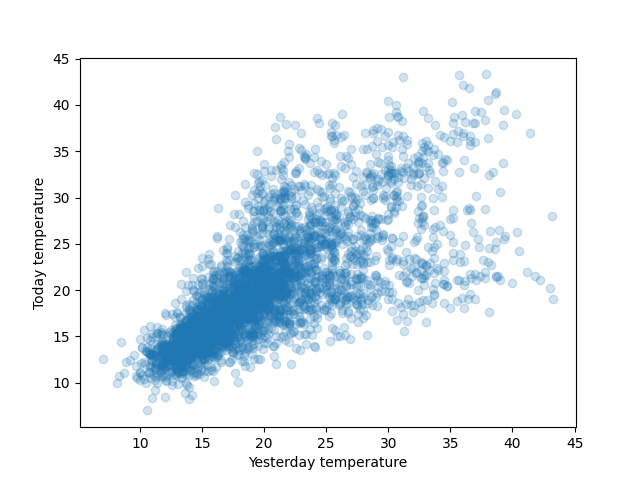
\includegraphics[width=\textwidth]{images/melbourne_temperature.png}
    \caption{Melbourne temperatures dataset}
    \label{fig:melbourne_temperature_data}
\end{figure}
Hereafter, the results of the four presented methods on the Melbourne dataset are reported, see figure \ref{fig:melbourne_quantiles_comparison} for a visualisation. Hyperparameter tuning have been optimised through cross validation, see \ref{appendix:cross_validation}.
\begin{figure}[!h]
    \begin{subfigure}[b]{0.5\linewidth}
      \centering
      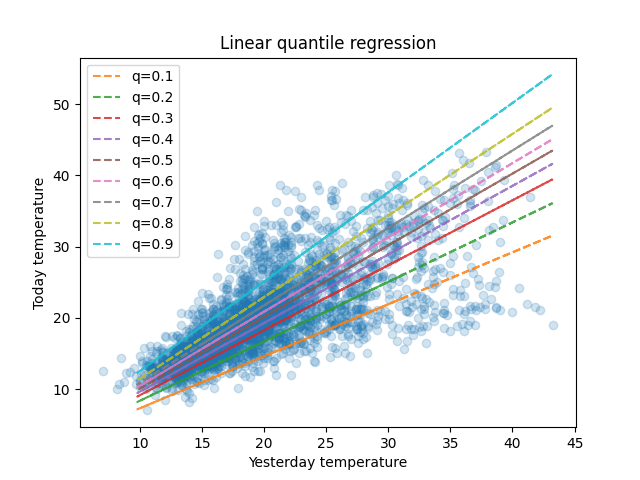
\includegraphics[width=1.1\textwidth]{images/melbourne_linear_quantile_regression.png} 
      \caption{Linear quantile regression} 
      \label{fig:melbourne_linear_quantile_regression} 
      \vspace{4ex}
    \end{subfigure}%% 
    \begin{subfigure}[b]{0.5\linewidth}
      \centering
      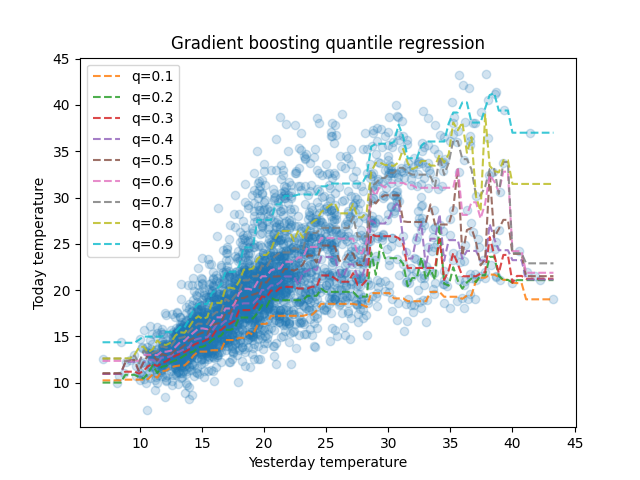
\includegraphics[width=1.1\textwidth]{images/melbourne_gradient_boosting_quantile_regression.png} 
      \caption{Gradient boosting quantile regression} 
      \label{fig:melbourne_gradient_boosting_quantile_regression} 
      \vspace{4ex}
    \end{subfigure} 
    \begin{subfigure}[b]{0.5\linewidth}
      \centering
      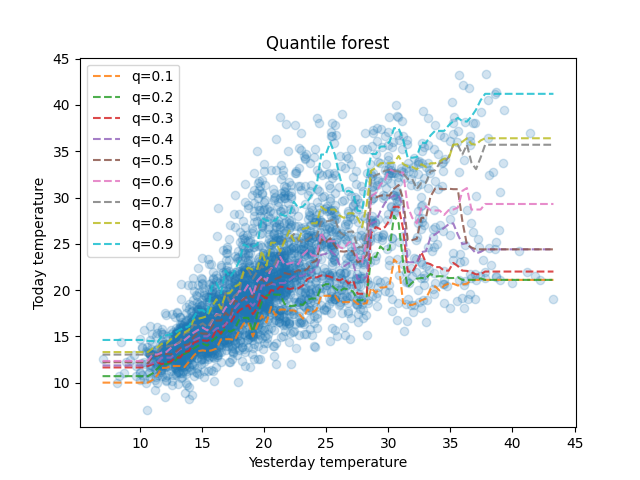
\includegraphics[width=1.1\textwidth]{images/melbourne_quantile_forest.png} 
      \caption{Quantile forest} 
      \label{fig:melbourne_quantile_forest} 
    \end{subfigure}%%
    \begin{subfigure}[b]{0.5\linewidth}
      \centering
      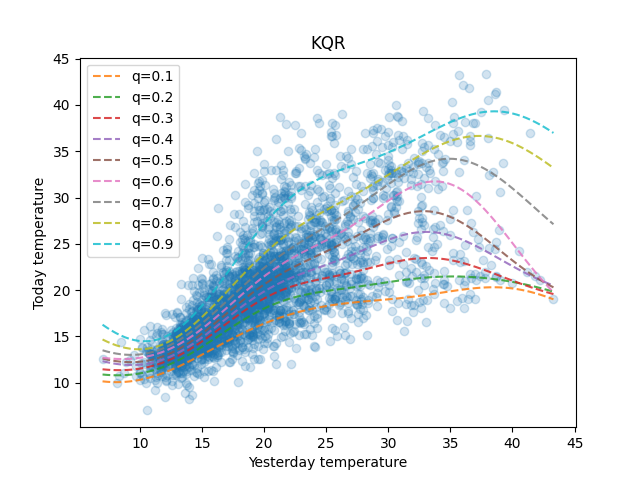
\includegraphics[width=1.1\textwidth]{images/melbourne_kernel_quantile_regression.png}
      \caption{Kernel quantile regression} 
      \label{fig:melborune_kernel_quantile_regression} 
    \end{subfigure} 
    \caption{Quantile regressors}
    \label{fig:melbourne_quantiles_comparison} 
  \end{figure}

% tables
\begin{table}[!h]
\caption{Pinball loss Melbourne data}
\begin{tabular}{lllll}
    \toprule
     & Linear qr & Gbm qr & Quantile forest & Kernel qr \\
    \midrule
    Pinball loss & 11.278895 & 10.317612 & 10.340842 & 10.031708 \\
    \bottomrule
    \end{tabular}
\end{table}

\begin{table}[!h]
    \caption{Pinball loss quantile-wise Melbourne data}
    \begin{tabular}{lllll}
    \toprule
    Quantiles & Linear qr & Gbm qr & Quantile forest & Kernel qr \\
    \midrule
    0.100000 & 0.710644 & 0.549232 & 0.562888 & 0.540235 \\
    0.200000 & 1.155014 & 0.938561 & 0.946712 & 0.903213 \\
    0.300000 & 1.417805 & 1.212671 & 1.222407 & 1.173803 \\
    0.400000 & 1.540108 & 1.399925 & 1.409293 & 1.367943 \\
    0.500000 & 1.574957 & 1.517281 & 1.484589 & 1.455849 \\
    0.600000 & 1.525114 & 1.498608 & 1.495474 & 1.447470 \\
    0.700000 & 1.397918 & 1.372183 & 1.362173 & 1.331503 \\
    0.800000 & 1.170140 & 1.115077 & 1.123195 & 1.096606 \\
    0.900000 & 0.787195 & 0.714075 & 0.734112 & 0.715085 \\
    \bottomrule
    \end{tabular}
\end{table}
As already pointed out, the quantile regression with q=0.5 corresponds to the standard regression problem, hence we can compare the proposed methods also in terms of the mean absolute error.
\begin{table}[!h]
\caption{Mean absolute error Melbourne data}
\begin{tabular}{lllll}
    \toprule
     & Linear qr & Gbm qr & Quantile forest & Kernel qr \\
    \midrule
    MAE & 3.253882 & 3.134805 & 3.095041 & 3.024336 \\
    \bottomrule
    \end{tabular}
\end{table}  
From these tables, we can see that kernel quantile regression outperformed the simple quantile regressor as well as the more complex models like quantile forest and gradient boosting quantile regression for the Melbourne temperatures dataset. Not only kernel quantile regression was the best in terms of total pinball loss but also the best in terms of each quantile pinball loss and mean absolute error.
Comparison has been carried out on further datasets, yielding similar conclusion as the one of above, to know more see \ref{appendix:quantile_regressor_extensive_comparison}.

We conclude this chapter with reporting the same kind of tables \ref{tab:kernel pinball comparison}, \ref{tab:kernel pinball comparison quantile-wise}, \ref{tab:kernel mae comparison} and figures \ref{fig:kernel quantile regressors comparison} comparing various kernel functions.

% tables
\begin{table}[!h]
    \caption{Kernels comparison pinball loss Melbourne data}
    \label{tab:kernel pinball comparison}
    \begin{center}
    \begin{tabular}{lll}
        \toprule
        & Kernel & Pinball loss
        \\
        \midrule
        & Gauss RBF &  10.031708 \\
        & Laplacian &  10.056884 \\
        & Gauss RBFxLaplacian & 10.150826 \\
        & Cosine & 16.253973    \\
        & Linear & 10.463867    \\
        & Polynomial & 11.238393     \\
        & Sigmoid & 16.253973            \\
        & Chi squared & 10.023732       \\
        & Matern & \textbf{10.021369}  \\
        & Periodic  & 15.946272\\
        \bottomrule
        \end{tabular}
    \end{center}
    \end{table}
    
\begin{table}[!h]
    \caption{Kernels comparison pinball loss quantile-wise Melbourne data}
    \label{tab:kernel pinball comparison quantile-wise}
    \begin{adjustbox}{width=\textwidth}
    \begin{tabular}{lllllllllll}
    \toprule
    Kernel/Quantiles & 0.1 & 0.2 & 0.3 & 0.4 & 0.5 & 0.6 & 0.7 & 0.8 & 0.9 \\
    \midrule
    Gauss RBF &  \textbf{0.540145} &
    \textbf{0.903193} &
    1.173627 &
    1.368022 &
    1.456053 &
    1.447470 &
    \textbf{1.331375} &
    1.096649 &
    0.715013 \\
    Laplacian &  0.542499 &
    0.906517 &
    1.177309 &
    1.371198 &
    1.462111 &
    1.453119 &
    1.340193 &
    \textbf{1.095991} &
    0.707947 \\
    Gauss RBFxLaplacian &0.545787 &
    0.915559 &
    1.189965 &
    1.387109 &
    1.479901 &
    1.475541 &
    1.350803 &
    1.101151 &
    \textbf{0.704922} \\
    Cosine & 0.755479 &
    1.343973 &
    1.802603 &
    2.123425 &
    2.307123 &
    2.367123 &
    2.262603 &
    1.971644 &
    1.320411 \\
    Linear &  0.565663 &
    0.947889 &
    1.250009 &
    1.437863 &
    1.506723 &
    1.478379 &
    1.358865 &
    1.135702 &
    0.782660   \\
    Polynomial &   0.542573 &
    0.908681 &
    1.178357 &
    \textbf{1.362351} &
    1.450249 &
    1.455228 &
    1.339822 &
    1.107768 &
    0.744118  \\
    Sigmoid &   0.755479 &
    1.343973 &
    1.802603 &
    2.123425 &
    2.307123 &
    2.367123 &
    2.262603 &
    1.971644 &
    1.320411          \\
    Chi squared &   0.541430 &
    0.906352 &
    1.173164 &
    1.358862 &
    \textbf{1.444130} &
    \textbf{1.440915} &
    1.332140 &
    1.100262 &
    0.726625     \\
    Matern &  0.541192 &
    0.903209 &
    \textbf{1.169543} &
    1.364430 &
    1.451248 &
    1.442511 &
    1.332522 &
    1.096750 &
    0.716226 \\
    Periodic  & 0.759452 &
    1.352747 &
    1.809921 &
    2.125765 &
    2.314718 &
    2.379657 &
    2.274711 &
    1.976768 &
    1.328630 \\
    \bottomrule
    \end{tabular}
    \end{adjustbox}
\end{table}

\begin{table}[!h]
    \caption{Kernels comparison mean absolute error Melbourne data}
    \label{tab:kernel mae comparison}
    \begin{center}
    \begin{tabular}{lll}
        \toprule
         & Kernel & MAE \\
        \midrule
        & Gauss RBF &  3.024336 \\
        & Laplacian &  3.038633 \\
        & Gauss RBFxLaplacian &  3.070812\\
        & Cosine &    4.849589 \\
        & Linear &     3.142352\\
        & Polynomial &     3.064472 \\
        & Sigmoid &      4.849589       \\
        & Chi squared &    \textbf{3.022778}    \\
        & Matern &  3.024517 \\
        & Periodic  & 4.880673 \\
        \bottomrule
        \end{tabular}
    \end{center}
    \end{table}  


% kernels figure

\begin{figure}[!h]
    \begin{subfigure}[b]{0.5\linewidth}
        \centering
        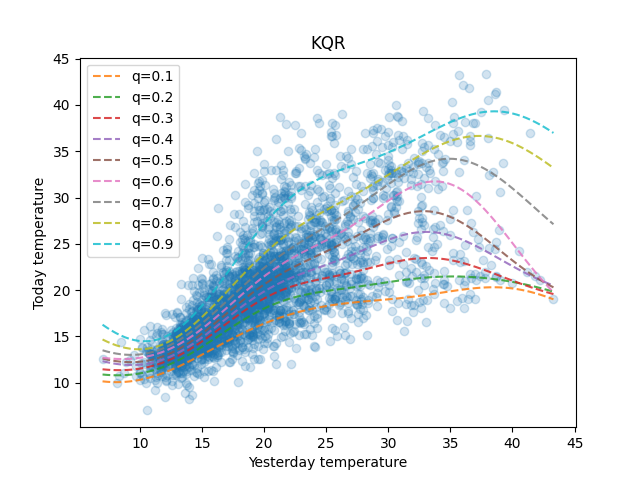
\includegraphics[width=1.1\textwidth]{images/melborune_gaussian_rbf_kernel_quantile_regression.png} 
        \caption{Gauss RBF} 
        \label{} 
        \vspace{4ex}
    \end{subfigure}%% 
    \begin{subfigure}[b]{0.5\linewidth}
        \centering
        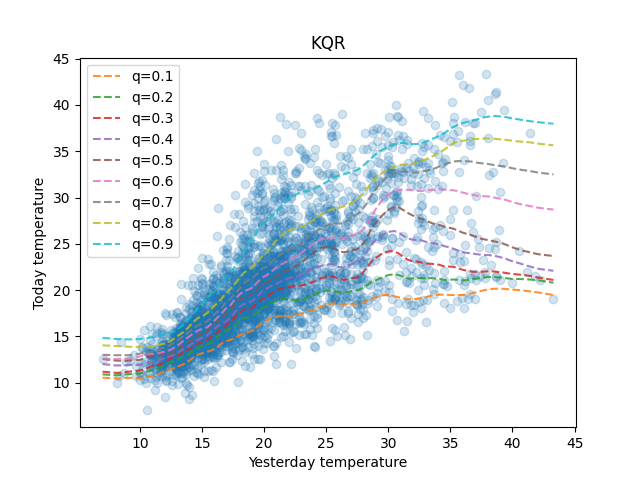
\includegraphics[width=1.1\textwidth]{images/melborune_laplacian_kernel_quantile_regression.png} 
        \caption{Laplacian} 
        \label{} 
        \vspace{4ex}
    \end{subfigure} 
    \begin{subfigure}[b]{0.5\linewidth}
        \centering
        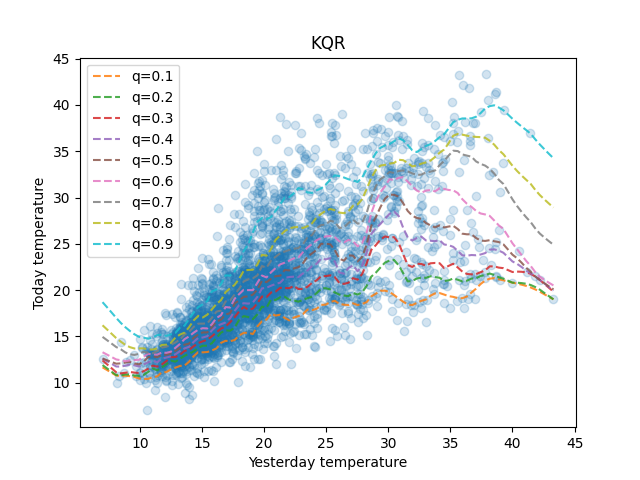
\includegraphics[width=1.1\textwidth]{images/melborune_gaussian_rbf_x_laplacian_kernel_quantile_regression.png} 
        \caption{Gauss RBFxLaplacian} 
        \label{} 
        \vspace{4ex}
    \end{subfigure}%%
    \begin{subfigure}[b]{0.5\linewidth}
        \centering
        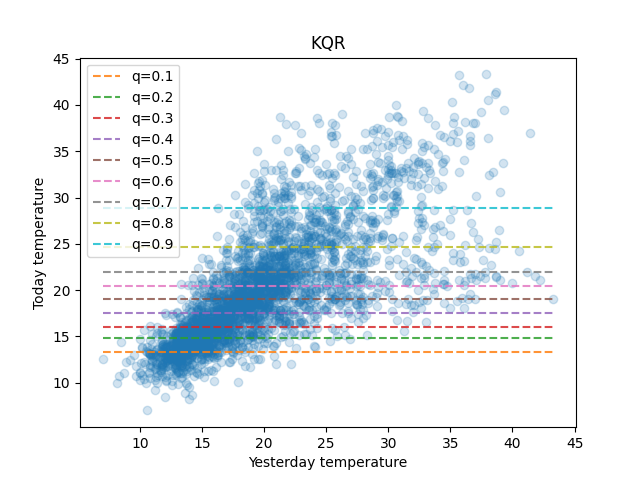
\includegraphics[width=1.1\textwidth]{images/melborune_cosine_kernel_quantile_regression.png}
        \caption{Cosine} 
        \label{} 
        \vspace{4ex}
    \end{subfigure} 
    \begin{subfigure}[b]{0.5\linewidth}
        \centering
        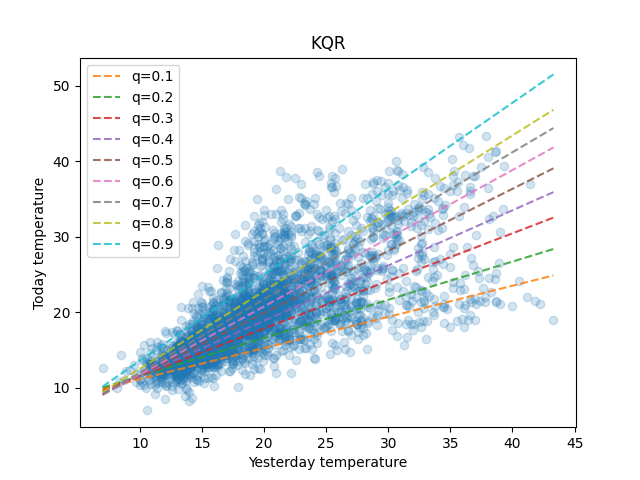
\includegraphics[width=1.1\textwidth]{images/melborune_linear_kernel_quantile_regression.png}
        \caption{Linear} 
        \label{} 
        \vspace{4ex}
    \end{subfigure} 
    \begin{subfigure}[b]{0.5\linewidth}
        \centering
        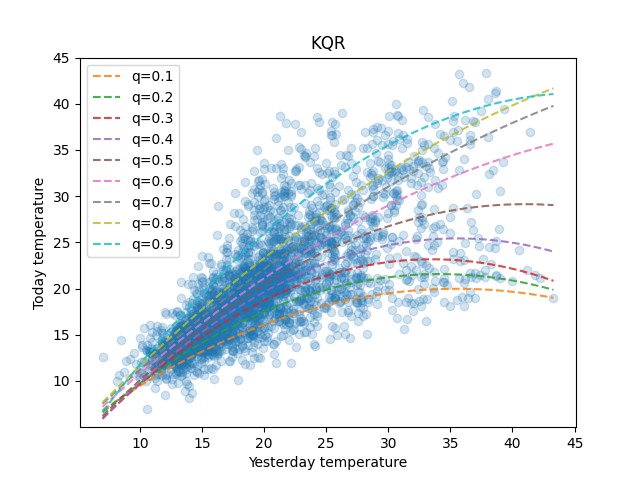
\includegraphics[width=1.1\textwidth]{images/melborune_polynomial_kernel_quantile_regression.png}
        \caption{Polynomial} 
        \label{} 
        \vspace{4ex}
    \end{subfigure} 
    \end{figure}


\begin{figure}[!h]\ContinuedFloat
    \begin{subfigure}[b]{0.5\linewidth}
        \centering
        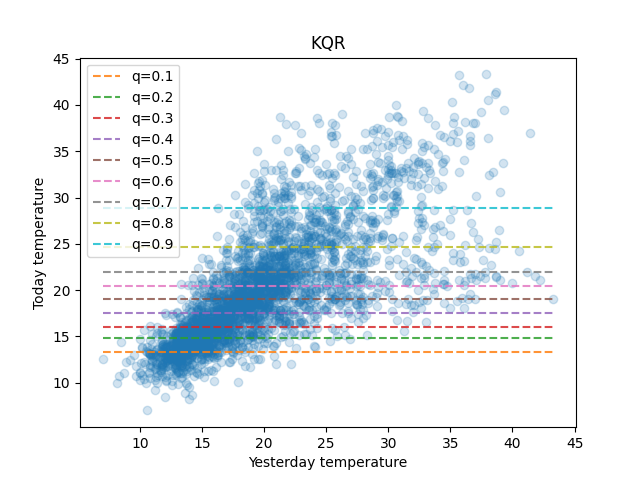
\includegraphics[width=1.1\textwidth]{images/melborune_sigmoid_kernel_quantile_regression.png}
        \caption{Sigmoid} 
        \label{} 
        \vspace{4ex}
    \end{subfigure} 
    \begin{subfigure}[b]{0.5\linewidth}
        \centering
        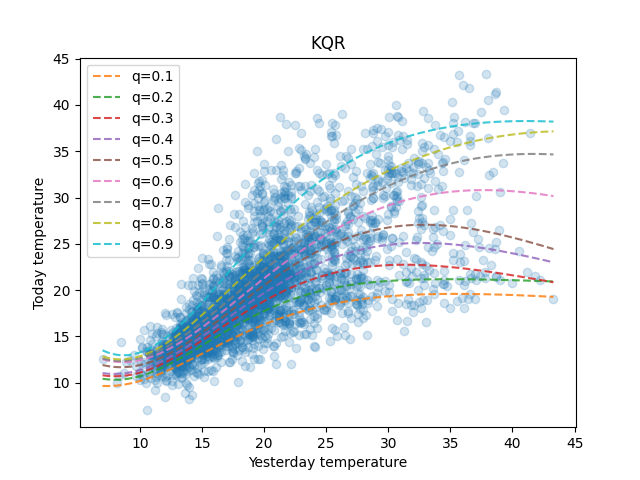
\includegraphics[width=1.1\textwidth]{images/melborune_chi_squared_kernel_quantile_regression.png}
        \caption{Chi squared} 
        \label{} 
        \vspace{4ex}
    \end{subfigure} 
    \begin{subfigure}[b]{0.5\linewidth}
        \centering
        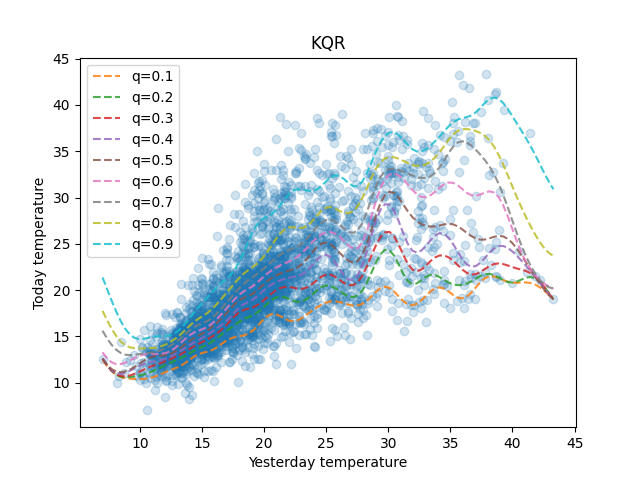
\includegraphics[width=1.1\textwidth]{images/melborune_matern_kernel_quantile_regression.png}
        \caption{Matern} 
        \label{} 
    \end{subfigure} 
    \begin{subfigure}[b]{0.5\linewidth}
        \centering
        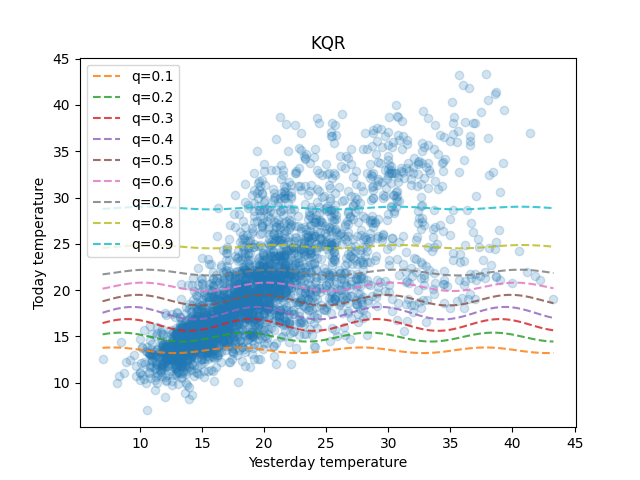
\includegraphics[width=1.1\textwidth]{images/melborune_periodic_kernel_quantile_regression.png}
        \caption{Periodic} 
        \label{} 
    \end{subfigure} 
    \caption{Kernel quantile regressors comparison}
    \label{fig:kernel quantile regressors comparison} 
\end{figure}

% \section{Kernel density estimation}
% - Explain the framework of kernel density estimation.

- Explain how it is applied in the literature.

- Extend to Conditional kernel density estimation
and how it is applied in the literature

- there is sample in sklearn kde, so we can use it to create a method of the kde class that computes its crps.

- Do a simple showcase with an example

% \section{Ensemble methods}
% - Explain the idea of ensemble methods.

- The most popular framework is based on
autoregressive processes, so explain their Theory
and how the procedure how they are used

- simple example

% \section{DMLP}
% %gluon nn
% % train a beta distribution to learn its parameters
% \section{DeepAR}


% \subsection{Kernel herding}
% Select the best point forecasting method and create a probabilistic forecast by modelling its model errors with kernel herding (do something like the residual bootstrap ensembles if it is meaningful and possible to implement).
